\documentclass{rapportClass} % Classe de document (rapport)



\title{Rapport de Projet}
\author{Hugo CLAVEILLE}
% -- Master 1 Informatique
\date{\today}




% Appliquer aussi aux pages de type 'plain' (début de chapitre, sommaire…)
% \fancypagestyle{plain}{
%   \fancyhf{}
%   \fancyhead[L]{Rapport de Projet}
%   \fancyhead[C]{M1 Informatique}
%   \fancyhead[R]{Hugo}
%   \fancyfoot[C]{\thepage}
%   \renewcommand{\headrulewidth}{0.4pt}
% }

\begin{document}

\begin{titlepage}
    \thispagestyle{empty} % pas d'en-tête/pied ici
    
    \begin{center}
        % Logo en haut
        
\includegraphics[width=1\textwidth]{logo.png}\\[2cm]
        
        % Titre
        {\Huge \textbf{Rapport de Projet}}\\[1cm]
        {\Large Software Engineering}\\[1cm]

        \vspace{1cm}
        % Auteur
        \textbf{Hugo CLAVEILLE}\\[0.5cm]
        
        % Sous-titre
        {\Large Master 1 Informatique}\\[2cm]
        
        % Date
        \vfill
        {\large \today}
    \end{center}
\end{titlepage}

\newpage
\thispagestyle{empty}
\tableofcontents
\newpage

% ======================================================================================================================
\chapter{Introduction}
Dans le cadre de l'Unités d'Enseignement de Software Engineering-2025, il nous a été demandé de réaliser un projet individuel
visant à étudier et implémenter des méthodes de transmission optimisée de données.
La transmission de tableaux d’entiers constitue un problème fondamental dans de nombreux systèmes
informatiques et réseaux, en particulier pour les applications nécessitant un échange rapide et
efficace de grandes quantités de données. Ce projet s’inscrit donc dans un contexte pratique où
la performance et l’efficacité des transferts d’information sont essentielles.

L’objectif est d’étudier différentes méthodes de compression de ces tableaux afin de réduire le nombre
de bits transmis tout en conservant un accès direct à chaque élément. La méthode choisie, appelée Bit Packing,
représente chaque entier avec le minimum de bits nécessaires, regroupés ensuite dans des entiers standards
pour la transmission. Deux variantes seront explorées : une autorisant l’écriture d’un entier compressé sur
deux entiers consécutifs, et une qui ne le permet pas. Le projet inclut également des benchmarks pour évaluer les gains de performance.

La gestion des débordements (overflow) est un aspect crucial de ce projet. En effet, lorsque les entiers à compresser
dépasse la capacité de bits allouée, il est nécessaire de mettre en place une stratégie efficace pour gérer ces cas.
La méthode choisie consiste à utiliser des entiers supplémentaires pour stocker les valeurs qui ne peuvent pas être représentées
dans le format compressé initial. Cette approche permet de maintenir l’intégrité des données tout en optimisant l’espace de stockage.






% ======================================================================================================================
\chapter{Présentation du problème et des objectifs}

L’objectif principal du projet est de concevoir et comparer deux méthodes de compression
de tableaux d’entiers en utilisant le principe du \textit{Bit Packing}.
Chaque entier est représenté à l’aide du nombre minimal de bits nécessaire, puis compacté dans un tableau
d’entiers 32 bits standard.

Deux variantes ont été implémentées :
\begin{itemize}
    \item \textbf{Méthode 1} : un entier compressé peut être réparti sur deux entiers consécutifs.
    \item \textbf{Méthode 2} : un entier compressé doit être contenu dans un seul entier.
\end{itemize}

\vspace{1em}
Le but de ces deux approches est de déterminer laquelle offre le meilleur compromis entre
temps de compression, temps de décompression et accessibilité directe à un élément donné.
Des benchmarks automatisés ont été mis en place pour comparer ces deux méthodes sur des tailles
de tableaux croissantes, distributions différentes ainsi que différents niveaux de compression (nombre de bits par entier).


% ======================================================================================================================
\chapter{Conception et Implémentation}

\section{Structure générale du projet}
Le projet est structuré autour de trois composants principaux :
\begin{itemize}
    \item Les classes \texttt{Method1Compressor} et \texttt{Method2Compressor} implémentant les deux méthodes de compression ;
    \item Un module de \textbf{benchmark} mesurant les performances pour différentes tailles de tableaux et valeurs de \texttt{maxbit} ;
    \item Un générateur de données permettant de produire des listes d'entiers selon plusieurs distributions (aléatoire uniforme, croissante, bruitée...).
\end{itemize}

\section{Methodes de compression}
Les deux classes \texttt{Method1Compressor} et \texttt{Method2Compressor} héritent d'une classe de base \texttt{CompressorBase}
qui définit l'interface commune pour la compression et la décompression.
Chaque classe implémente les méthodes \texttt{compress()}, \texttt{decompress()} et \texttt{get()} selon la logique spécifique à chaque méthode.

Les deux méthodes utilisent des algorithmes différents pour gérer la répartition des bits et l'accès aux éléments compressés que nous détaillerons ci-dessous.
Nous traiterons plus tard de la gestion des débordements (overflow) lorsque les entiers à compresser dépassent la capacité allouée.
Chaque entier compressé utilisant un nombre de bits inférieur ou égal à \texttt{maxbit} est annoté d'un préfixe 0 avant sa représentation binaire.
Si l'entier dépasse cette capacité, il est annoté d'un préfixe 1 et stocké dans une structure dédiée aux débordements, decrite dans la section suivante.
\subsection{Méthode 1 : Entiers scindables}
Dans cette méthode, un entier compressé peut être réparti sur deux entiers consécutifs.
Cela permet une utilisation plus efficace de l'espace lorsque les entiers à compresser ne s'alignent pas parfaitement avec les limites des entiers 32 bits.
Par exemple, si chaque entier compressé utilise 10 bits, trois entiers compressés peuvent être stockés dans un entier 32 bits,
et le quatrième sera scindé entre le premier et le deuxième entier suivant. (voir Figure 3.1)
Cette approche maximise l'utilisation de chaque bit disponible, mais complique légèrement la logique d'accès aux éléments compressés.
\begin{figure}[h!]
    \centering
    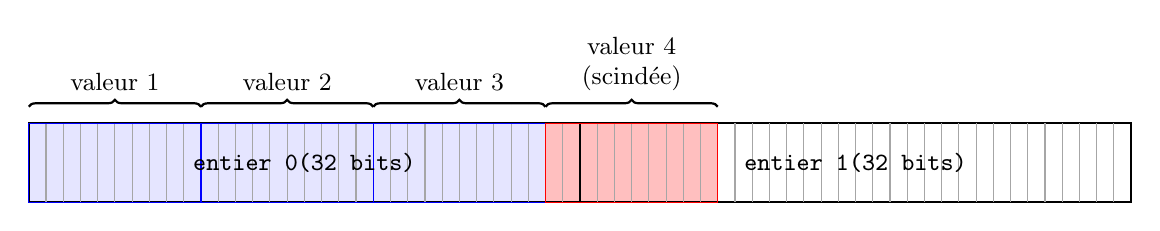
\begin{tikzpicture}[font=\small]
        % paramètres (mêmes logique)
        \def\wordw{7.0}
        \def\wordh{1.0}
        \def\k{10} % nombre de bits par entier
        \def\nbits{32}
        \def\scaleBit{\wordw/\nbits}
        \def\words{1}

        % Colorier champs : première valeur complète dans mot 0
        \filldraw[fill=blue!10,draw=blue!100] (0*\scaleBit,0) rectangle ++(\k*\scaleBit,-\wordh);
        % deuxième valeur 
        \filldraw[fill=blue!10,draw=blue!100] (\k*\scaleBit,0) rectangle ++(\k*\scaleBit,-\wordh);
        % troisième valeur 
        \filldraw[fill=blue!10,draw=blue!100] (2*\k*\scaleBit,0) rectangle ++(\k*\scaleBit,-\wordh);
        % quatrième valeur (scindée)
        \filldraw[fill=red!25,draw=red!100] (3*\k*\scaleBit,0) rectangle ++(\k*\scaleBit,-\wordh);



        % dessiner mots
        \foreach \w in {0,...,\words} {
            \draw[thick] (\w*\wordw,0) rectangle ++(\wordw,-\wordh);
            \pgfmathtruncatemacro{\maxbits}{\nbits-1}
            \foreach \b in {1,...,\maxbits} {
                \draw[gray!70] (\w*\wordw+\b*\scaleBit,0) -- ++(0,-\wordh);
            }
        }

        \draw[blue!100] (0*\k*\scaleBit,0) rectangle ++(\k*\scaleBit,-\wordh);
        \draw[blue!100] (1*\k*\scaleBit,0) rectangle ++(\k*\scaleBit,-\wordh);
        \draw[blue!100] (2*\k*\scaleBit,0) rectangle ++(\k*\scaleBit,-\wordh);
        \draw[red!100] (3*\k*\scaleBit,0) rectangle ++(\k*\scaleBit,-\wordh);

        % noms des mots
        \foreach \w in {0,1} {
            \node at (\w*\wordw + \wordw/2, -\wordh/2) {\texttt{entier \w (32 bits)}};
        }

        % accolades / labels : pour la valeur 3 (scindée)
        % partie 1 (dans word0)
        \draw [decorate,decoration={brace,raise=6pt},thick] (0,0) -- ++(\k*\scaleBit,0) node[midway,above=8pt]{valeur 1};
        \draw [decorate,decoration={brace,raise=6pt},thick] (\k*\scaleBit * 1,0) -- ++(\k*\scaleBit,0) node[midway,above=8pt]{valeur 2};
        \draw [decorate,decoration={brace,raise=6pt},thick] (\k*\scaleBit * 2,0) -- ++(\k*\scaleBit,0) node[midway,above=8pt]{valeur 3};
        % la quartième valeur
        % \draw [decorate,decoration={brace,raise=6pt},thick] (\k*\scaleBit * 3,0) -- ++(\k*\scaleBit,0) node[midway,above=8pt]{valeur 4 \\ (scindée)};
        \draw [decorate,decoration={brace,raise=6pt},thick]
            (\k*\scaleBit * 3,0) -- ++(\k*\scaleBit,0)
            node[midway,above=8pt,align=center]{valeur 4 \\ (scindée)};    \foreach \v in {0,...,3} {
            % \draw[decorate,decoration={brace,raise=6pt},thick] (\k * \scaleBit * \v,0) -- ++(\k*\scaleBit * (\v + 1),0) node[midway,above=8pt]{valeur 1 (10 bits)};
        }

    \end{tikzpicture}

    \caption{Méthode 1 — un entier peut être scindé entre deux mots (ici : 2 + 8 bits).}
\end{figure}

\subsection{Méthode 2 : Entiers non scindables}
Dans cette méthode, chaque entier compressé doit être entièrement contenu dans un seul entier 32 bits.
Cela simplifie l'accès aux éléments compressés, car chaque entier peut être récupéré directement sans
avoir à gérer la logique de scission entre deux entiers. Cependant, cette approche peut entraîner une utilisation moins efficace de l'espace,
car certains bits dans les entiers 32 bits peuvent rester inutilisés si le nombre de bits par entier compressé ne s'aligne pas parfaitement avec 32.
\begin{figure}[h!]
    \centering
    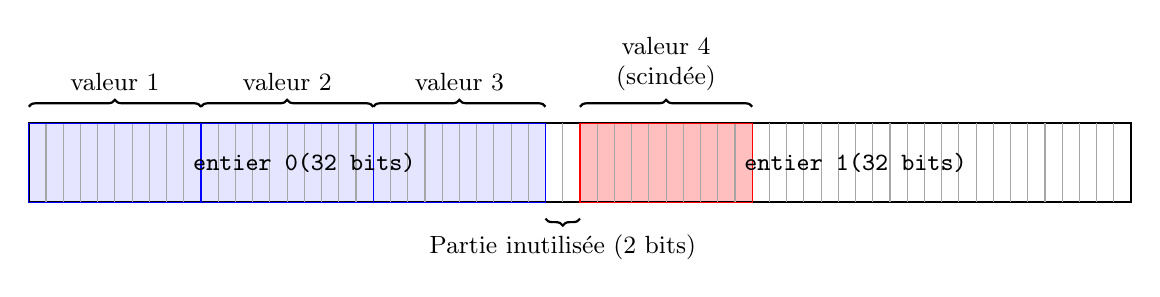
\begin{tikzpicture}[font=\small]
        % paramètres (mêmes logique)
        \def\wordw{7.0}
        \def\wordh{1.0}
        \def\k{10} % nombre de bits par entier
        \def\nbits{32}
        \def\scaleBit{\wordw/\nbits}
        \def\words{1}

        % Colorier champs : première valeur complète dans mot 0
        \filldraw[fill=blue!10,draw=blue!100] (0*\scaleBit,0) rectangle ++(\k*\scaleBit,-\wordh);
        % deuxième valeur 
        \filldraw[fill=blue!10,draw=blue!100] (\k*\scaleBit,0) rectangle ++(\k*\scaleBit,-\wordh);
        % troisième valeur 
        \filldraw[fill=blue!10,draw=blue!100] (2*\k*\scaleBit,0) rectangle ++(\k*\scaleBit,-\wordh);
        % quatrième valeur (scindée)
        \filldraw[fill=red!25,draw=red!100] (3*\k*\scaleBit + 2*\scaleBit,0) rectangle ++(\k*\scaleBit,-\wordh);



        % dessiner mots
        \foreach \w in {0,...,\words} {
            \draw[thick] (\w*\wordw,0) rectangle ++(\wordw,-\wordh);
            \pgfmathtruncatemacro{\maxbits}{\nbits-1}
            \foreach \b in {1,...,\maxbits} {
                \draw[gray!70] (\w*\wordw+\b*\scaleBit,0) -- ++(0,-\wordh);
            }
        }

        \draw[blue!100] (0*\k*\scaleBit,0) rectangle ++(\k*\scaleBit,-\wordh);
        \draw[blue!100] (1*\k*\scaleBit,0) rectangle ++(\k*\scaleBit,-\wordh);
        \draw[blue!100] (2*\k*\scaleBit,0) rectangle ++(\k*\scaleBit,-\wordh);
        \draw[red!100] (3*\k*\scaleBit + 2*\scaleBit,0) rectangle ++(\k*\scaleBit,-\wordh);

        % noms des mots
        \foreach \w in {0,1} {
            \node at (\w*\wordw + \wordw/2, -\wordh/2) {\texttt{entier \w (32 bits)}};
        }

        % accolades / labels : pour la valeur 3 (scindée)
        % partie 1 (dans word0)
        \draw [decorate,decoration={brace,raise=6pt},thick] (0,0) -- ++(\k*\scaleBit,0) node[midway,above=8pt]{valeur 1};
        \draw [decorate,decoration={brace,raise=6pt},thick] (\k*\scaleBit * 1,0) -- ++(\k*\scaleBit,0) node[midway,above=8pt]{valeur 2};
        \draw [decorate,decoration={brace,raise=6pt},thick] (\k*\scaleBit * 2,0) -- ++(\k*\scaleBit,0) node[midway,above=8pt]{valeur 3};
        % la quartième valeur
        % \draw [decorate,decoration={brace,raise=6pt},thick] (\k*\scaleBit * 3,0) -- ++(\k*\scaleBit,0) node[midway,above=8pt]{valeur 4 \\ (scindée)};
        \draw [decorate,decoration={brace,raise=6pt},thick]
            (\k*\scaleBit * 3 + 2*\scaleBit,0) -- ++(\k*\scaleBit,0)
            node[midway,above=8pt,align=center]{valeur 4 \\ (scindée)};    \foreach \v in {0,...,3} {
            % \draw[decorate,decoration={brace,raise=6pt},thick] (\k * \scaleBit * \v,0) -- ++(\k*\scaleBit * (\v + 1),0) node[midway,above=8pt]{valeur 1 (10 bits)};
        }


        \draw [decorate,decoration={brace,mirror,raise=6pt},thick]
            (\k*\scaleBit * 3,-\wordh) -- ++(2*\scaleBit,0)
            node[midway,below=8pt]{Partie inutilisée (2 bits)};

    \end{tikzpicture}

    \caption{Méthode 1 — un entier peut être scindé entre deux mots (ici : 2 + 8 bits).}
\end{figure}

% \begin{itemize}
%     \item \textbf{Méthode 1} : On stoque les entiers compressés en permettant qu’un entier puisse être réparti sur deux entiers consécutifs.


%     \item \textbf{Méthode 2} : Lorsqu’un entier dépasse la taille maximale définie par \texttt{maxbit}, il est stocké dans un entier supplémentaire.
%     Cette approche permet d’assurer la cohérence de la décompression sans perte de données.
% \end{itemize}

% ======================================================================================================================
\section{Gestion des débordements}
A FAIRE ------------------------------
La gestion des débordements est gérée diferémment selon la méthode choisie, mais utilisent le meme principe de detection.
Lorsqu’un entier à compresser dépasse la capacité maximale définie par \texttt{maxbit}, on stoque son indice 
\subsection{Méthode 1}
Lorsqu’un entier dépasse la taille maximale définie par \texttt{maxbit}, on le stoque en fin de chaine
dans un tableau dédié aux débordements. Un indicateur spécial est utilisé dans le flux compressé pour signaler la présence d’un débordement.
Lors de la décompression, si cet indicateur est rencontré, la valeur correspondante est récupérée depuis le tableau des débordements.
\subsection{Méthode 2}
% \begin{itemize}
%     \item \textbf{Méthode 1} : Lorsqu’un entier dépasse la taille maximale définie par \texttt{maxbit}, on le stoque en fin de chaine 

%     \item \textbf{Méthode 2} : Lorsqu’un entier dépasse la taille maximale définie par \texttt{maxbit}, il est stocké dans un entier supplémentaire.
%     Cette approche permet d’assurer la cohérence de la décompression sans perte de données.
% \end{itemize}
% Lorsqu’un entier dépasse la taille maximale définie par \texttt{maxbit}, il est stocké dans un entier supplémentaire.
% Cette approche permet d’assurer la cohérence de la décompression sans perte de données.



% ======================================================================================================================
\chapter{Résultats et Analyse des Benchmarks}

\section{Méthodologie de Benchmark}

Afin d’évaluer les performances des deux méthodes de compression développées, une campagne de
mesures automatisées a été réalisée à l’aide d’un script Python dédié.  
Chaque configuration est définie par quatre paramètres principaux :
\begin{itemize}
    \item le \underline{nombre de bits} utilisés pour encoder chaque entier (\texttt{max\_bits}) ;
    \item la \underline{taille du tableau} d’entrée (\texttt{n}) ;
    \item la \underline{méthode de compression} (\texttt{method1} ou \texttt{method2}).
    \item le \underline{type de distribution} des entiers (\texttt{aléatoire uniforme}, \texttt{croissante} ou \texttt{bruitée}).
\end{itemize}

\vspace{1em}
Pour chaque combinaison de paramètres, plusieurs itérations sont effectuées afin d’obtenir des
moyennes représentatives des temps de traitement.  
Les trois opérations principales sont mesurées séparément :
\begin{itemize}
    \item \textbf{Compression} : transformation du tableau d’entiers bruts en format compressé.
    \item \textbf{Décompression} : restitution du tableau original à partir du format compressé.
    \item \textbf{Accès direct} (\texttt{get}) : récupération aléatoire d’éléments sans décompression complète.
\end{itemize}

\vspace{1em}
Chaque test est répété plusieurs fois pour éliminer les effets de cache ou d’aléa d’exécution.  
Les résultats sont sauvegardés dans un fichier CSV brut, puis agrégés en moyennes pour faciliter l’analyse
et la génération de graphiques.  

\section{Résultats Expérimentaux}

Aprés avoir exécuté les benchmarks selon la méthodologie décrite précédemment, nous pouvons maintenant nous intéresser aux résultats obtenus.
Dans un premier temps, nous allons examiner les temps de compression et de décompression ainsi que les temps d’accès direct aux éléments compressés
moyen pour chaque méthode sans tenir compte des différentes distributions de données ni du nombre de bits d'encodage.

% Les benchmarks ont été menés sur différentes tailles de tableaux (100, 1 000 et 10 000 éléments) et
% pour un nombre de bits variant de 4 à 20.  
% Les graphiques suivants présentent l’évolution des temps moyens en fonction de ces paramètres.  
% Ils permettent d’identifier les comportements distincts des deux méthodes.

\subsection{Temps de compression et de décompression}

Les temps de compression augmentent naturellement avec la taille du tableau et la complexité du codage
(nombre de bits utilisés).  
Mais, malgré ce qu'on pourrait attendre, la \textbf{Méthode 1} montre des performances nettement supérieures
à la \textbf{Méthode 2} pour des tailles de tableaux plus importantes.  
Cela s’explique par la flexibilité offerte par la possibilité de scinder les entiers entre deux mots,
ce qui optimise l’utilisation de l’espace et réduit le nombre d’opérations nécessaires.
Voir figure \ref{fig:global_compression_times}.

\begin{figure}[h!]
    \centering
    \begin{tikzpicture}
    \begin{axis}[
        width=1\textwidth,
        height=0.5\textwidth,
        xlabel={Taille du tableau $n$},
        ylabel={Temps (ms)},
        xmode=log,              % <-- active l’échelle logarithmique
        log basis x={10},       % base 10 (ou 2)
        xtick={100,1000,10000}, % valeurs affichées sur l’axe
        legend pos=north west,
        grid=major
    ]

    % Méthode 1
    \addplot table[x=n, y=compress_decompress_time_avg, col sep=comma] {../out/data/moy_method1.csv};
    % \addplot table[x=n, y=compress_decompress_time_avg, col sep=comma] {../moy_all.csv};
    \addlegendentry{Compression/Décompression - Méthode 1}

    \addplot table[x=n, y=compress_decompress_time_avg, col sep=comma] {../out/data/moy_method2.csv};
    \addlegendentry{Compression/Décompression - Méthode 2}

    \end{axis}
    \end{tikzpicture}
    \caption{Performance de la Méthode 1 : temps de compression et décompression moyen en fonction de la taille du tableau.}
    \label{fig:global_compression_times}
\end{figure}


\subsection{Temps d’accès direct (\texttt{get})}

La mesure des accès aléatoires est clairement etrange, le temps moyen d'accès direct via la méthode \texttt{get()}
semble diminuer avec l'augmentation de la taille du tableau, ce qui est contre-intuitif.  
Cela pourrait être dû a la modification du nombre de bits utilisés pour l'encodage. Nous y reviendrons plus tard.
\begin{figure}[H]
    \centering
    \begin{tikzpicture}
    \begin{axis}[
        width=1\textwidth,
        height=0.5\textwidth,
        xlabel={Taille du tableau $n$},
        ylabel={Temps moyen d'accès (µs)},
        xmode=log,              % <-- active l’échelle logarithmique
        log basis x={10},       % base 10 (ou 2)
        xtick={100,1000,10000}, % valeurs affichées sur l’axe
        legend pos=south west,
        grid=major
    ]

    % Méthode 1
    \addplot table[x=n, y=get_time_avg, col sep=comma] {../out/data/moy_get_method1.csv};
    % \addplot table[x=n, y=compress_decompress_time_avg, col sep=comma] {../moy_all.csv};
    \addlegendentry{Accès direct - Méthode 1}

    \addplot table[x=n, y=get_time_avg, col sep=comma] {../out/data/moy_get_method2.csv};
    \addlegendentry{Accès direct - Méthode 2}

    \end{axis}
    \end{tikzpicture}
    \caption{Performance de la Méthode 1 : temps moyen d’accès direct en fonction de la taille du tableau.}
    \label{fig:global_get_times}
\end{figure}

\section{Resultats détaillés par distribution et nombre de bits}
Afin de mieux comprendre les performances des deux méthodes, nous avons analysé les résultats
en fonction des différentes distributions de données et du nombre de bits utilisés pour l’encodage.  
\subsection{Nombre de bits}

L'impact du nombre de bits sur les performances est significatif. En général, une augmentation du nombre de bits
utilisés pour l'encodage conduit à une amélioration des temps de compression et de décompression, mais peut
également augmenter le temps d'accès direct.  
Les graphiques suivants illustrent ces variations en fonction de la taille du tableau et de la méthode utilisée.

% heatmap
\begin{figure}[H]
    \centering
    \begin{tikzpicture}
    \begin{axis}[
        width=1\textwidth,
        height=0.5\textwidth,
        xlabel={Taille du tableau $n$},
        ylabel={Nombre de bits},
        colorbar,
        colormap/viridis,
        point meta min=0,
        point meta max=50,
        grid=major
    ]

    % Méthode 1
    \addplot [
        matrix plot*,
        mesh/cols=3,  % 3 valeurs de n
        point meta=explicit
    ] table     [
        x=n,
        y=max_bits,
        meta=time_avg,
        col sep=comma
    ] {../out/data/heatmap_method1.csv};
    \addlegendentry{Méthode 1}

    \end{axis}
    \end{tikzpicture}
    \caption{Heatmap des performances en fonction de la taille du tableau et du nombre de bits utilisés.}
    \label{fig:heatmap_performance}
\end{figure}








\section{Visualisations et Interprétation}

Les graphiques 2D permettent une lecture intuitive de l’évolution des performances pour chaque paramètre.  
Afin de mieux comprendre les interactions entre la taille du tableau, le nombre de bits et le temps d’exécution,
des \textbf{graphiques 3D} et \textbf{heatmaps} ont été utilisés.  
Ces visualisations offrent une représentation synthétique des zones de performance optimale,
et mettent en évidence les compromis entre compacité et vitesse.

Par exemple, les heatmaps montrent clairement que la \textbf{Méthode 2} est plus efficace pour des tailles modérées
et un encodage limité (moins de 12 bits), tandis que la \textbf{Méthode 1} devient plus intéressante lorsque la
taille des données et le nombre de bits augmentent.

\section{Discussion}

L’analyse des résultats suggère que le choix entre les deux méthodes dépend du contexte d’utilisation :
\begin{itemize}
    \item pour des tableaux de taille moyenne et un besoin de vitesse, la \textbf{Méthode 2} est à privilégier ;
    \item pour des grands volumes ou des tailles de mots variables, la \textbf{Méthode 1} offre un meilleur compromis
          entre compacité et flexibilité.
\end{itemize}

L’intégration d’une stratégie adaptative, sélectionnant automatiquement la méthode la plus appropriée selon
le profil des données, pourrait constituer une amélioration future du système.





\chapter{Benchmark}
Les benchmarks ont été réalisés automatiquement pour des tailles de tableau $n = 100, 1000 et 10000$
et des valeurs de \texttt{maxbit} comprises entre 4 et 20 (pas de 2).
Chaque exécution mesure :
\begin{itemize}
    \item le temps de compression,
    \item le temps de décompression,
    \item le temps moyen d’accès via la méthode \texttt{get()}.
\end{itemize}
Les résultats sont enregistrés dans un fichier JSON et agrégés dans un CSV pour exploitation graphique.







% ======================================================================================================================
% ======================================================================================================================
\chapter{Conclusion et Perspectives}

Ce projet a permis de comparer deux méthodes de compression d'entiers basées sur le principe
du \textit{Bit Packing}. Les résultats des benchmarks montrent que le compromis entre performance
et complexité dépend fortement du contexte d’utilisation.

Les perspectives d’amélioration incluent :
\begin{itemize}
    \item l’utilisation de parallélisme pour accélérer la compression,
    \item l’intégration d’un mode adaptatif choisissant automatiquement la méthode la plus efficace,
    \item l’ajout d’un module de visualisation temps réel des performances.
\end{itemize}
% ======================================================================================================================

\chapter{Résultats expérimentaux}

\section{Temps de compression}
% ton graphique ici

\section{Temps de décompression}
% même style de graphique

\section{Temps moyen d'accès (get())}
% encore un graphique

\section{Analyse des résultats}
Les résultats montrent que la méthode 1, bien que plus coûteuse en mémoire dans certains cas,
offre de meilleures performances en compression et en décompression lorsque la taille du tableau augmente.
La méthode 2 reste plus stable, mais devient moins efficace pour de grands volumes de données.



\chapter{Résultats des Benchmarks}

\section{Temps de compression}

\begin{figure}[h!]
\centering
\begin{tikzpicture}
\begin{axis}[
    xlabel={Taille du tableau $n$},
    ylabel={Temps de compression (ms)},
    legend pos=north west,
    width=0.8\textwidth,
    height=0.5\textwidth,
    grid=major,
    cycle list name=color list
]

% Méthode 1
% \addplot table[x=n, y=compress_time_avg, col sep=comma, select expr={\thisrow{method}=="method1"}]{bench_results_agg.csv};
\addlegendentry{Method 1}
\addplot table[
    x=n, y=compress_time_avg,
    col sep=comma,
    row predicate/.code={
        \ifnum\pdfstrcmp{\thisrow{method}}{method1}=0
            \edef\pgfmathresult{1}
        \else
            \edef\pgfmathresult{0}
        \fi
    }
] {../out/data/bench_results_agg.csv};

% Méthode 2
% \addplot table[x=n, y=compress_time_avg, col sep=comma, select expr={\thisrow{method}=="method2"}]{bench_results_agg.csv};
% \addlegendentry{Method 2}

\end{axis}
\end{tikzpicture}
\caption{Comparaison des temps de compression entre les deux méthodes selon la taille du tableau.}
\end{figure}


% \lipsum[1-5] % Texte factice pour l'introduction
% \chapter{Introduction}
% Ici tu présentes le contexte et les objectifs de ton projet.


% \chapter{Travaux Réalisés}
% Explique la méthodologie, les outils utilisés, ton code, etc.

% \section{Outils utilisés}
% Exemple d’outils : Python, C++, Git, Docker...

% \section{Exemple de code}
% Voici un exemple en LaTeX :
% \begin{lstlisting}[language=C++]
% #include <iostream>
% using namespace std;

% int main() {
%     cout << "Hello World!";
%     return 0;
% }
% \end{lstlisting}	

% \chapter{Résultats}
% Explique ce que tu as obtenu.

% \chapter{Conclusion et Perspectives}
% Résumé de ton projet et idées pour la suite.

\end{document}
